\documentclass[aspectratio=169,notes]{beamer}
\usepackage{lmodern}
\usepackage[T1]{fontenc}
\usepackage{textcomp}
\usepackage{animate}
\usepackage{underscore}
\usepackage{pdfpc-commands}
\usepackage{xmpmulti}
\usepackage{multimedia}
\usepackage{epstopdf}
\usepackage{hyperref}
\usepackage{listings}
\usepackage{tikz}
\usetikzlibrary{shadows}
\usepackage{xkeyval}
\usepackage{todonotes}
\presetkeys{todonotes}{inline}{}
\defbeamertemplate{description item}{align left}{\insertdescriptionitem\hfill}
\usetheme{metropolis}					 % Use metropolis theme
\usepackage[
    backend=biber,
    url=true, 
	style=numeric,
    doi=true,
    eprint=false
]{biblatex}
\addbibresource{biblatex-examples.bib}

\title{All Spreadsheets must Die}
\date{\today}
\author{Robert Schadek}
\begin{document}
	\maketitle

	\section{Getting started}
	\begin{frame}{A random list of languages we love to hate}
		\begin{itemize}
			\item Rust
			\item Go
			\item C++
			\item JavaScript
			\item Typescript
		\end{itemize}
		\todo{replace itemize with logos}
	\end{frame}

	\note[itemize]{
		\item There are all these languages we like to hate.
		\item Many of them are good, many are more popular.
		\item Many might even be better.
		\item But we are missing something
	}

	\begin{frame}{Hating by numbers}
		\begin{description}
			\item[C++] $4.4 Million$ (2015)
			\item[C] $1.9 Million$ (2015)
			\item[Java] $9 Million$ (2009)	
			\item[JS] $10 Million$ (2018)
		\end{description}
	\end{frame}
	
	\begin{frame}
		\begin{center}
		\huge
		These are all small fish\\[2cm]
		\pause
		\textbf{Excel} $750 Million$ (2016)
		\end{center}
	\end{frame}

	\begin{frame}[fragile]
		\begin{center}
		
\includegraphics[width=0.6\textwidth]{skepical.jpg}
		\end{center}
	\end{frame}

	\begin{frame}[fragile]{Oh, but it is \hfill{} \cite{GOTO201638:online}}
		\begin{center}
		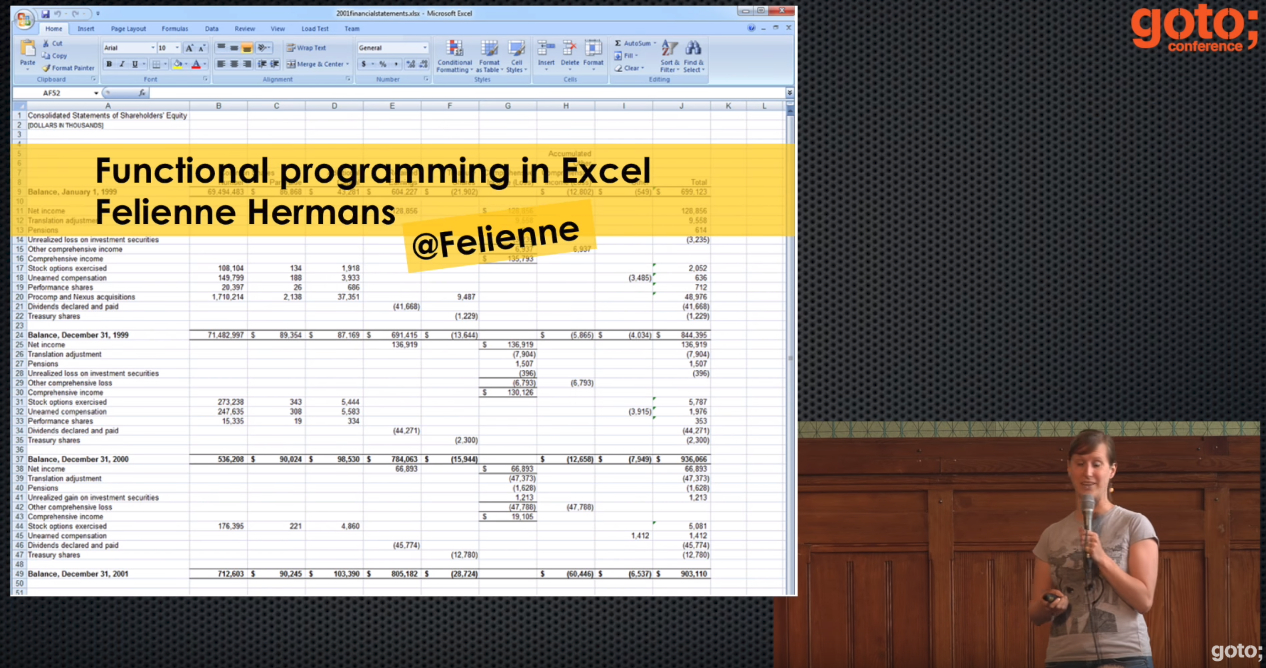
\includegraphics[width=1.0\textwidth]{functionalexcel.jpg}
		\end{center}
	\end{frame}

	\section{A little bit of Spreadsheet bashing}
	\begin{frame}[fragile]{See the code is difficult}
		\begin{center}
		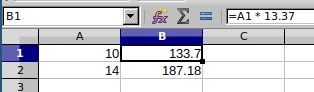
\includegraphics[width=1.0\textwidth]{excelseeingcode.jpg}
		\end{center}
	\end{frame}

	\begin{frame}[fragile]{Dynamic Types}
		\begin{center}
		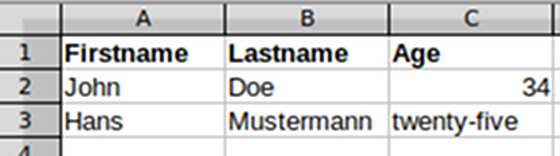
\includegraphics[width=1.0\textwidth]{exceldynamic.jpg}
		\end{center}
	\end{frame}

	\begin{frame}[fragile]{Dynamic Types}
		\begin{center}
		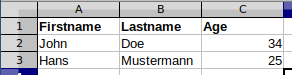
\includegraphics[width=1.0\textwidth]{exceldynamic2.jpg}
		\end{center}
	\end{frame}

	\begin{frame}[fragile]{Dynamic Types}
		\begin{center}
		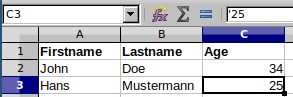
\includegraphics[width=1.0\textwidth]{exceldynamic3.jpg}
		\end{center}
	\end{frame}

	\begin{frame}[fragile]
		\begin{center}
		
\includegraphics[width=0.6\textwidth]{boyholdingfart.jpg}
		\end{center}
	\end{frame}

	\begin{frame}[fragile]{git blame}
		\begin{center}
			\huge
			git blame\\[2cm]
			\pause
			lets not go there\footnote{we will just become sad}
		\end{center}
	\end{frame}

	\begin{frame}[fragile]{Code refactoring}
		\begin{itemize}
			\item \lstinline@=SUM(1,2)@ \pause
			\item equal, identifier, lparen, int(1), comma, int(2), comma, int(3), rparen
			\item set excel locale to de\_DE
			\item \lstinline@=SUM(1,2)@ \pause
			\item equal, identifier, lparen, float(1.2), rparen
		\end{itemize}
	\end{frame}

	\begin{frame}[fragile]{Bits and pieces}
		\begin{itemize}
			\item Knowledge silos
			\item Slow	
			\item No separation between data and code
			\item Access management $\dots$ anybody
		\end{itemize}
	\end{frame}

	\begin{frame}[fragile]{(Typical) Spreadsheet Lifecycle}
		\begin{enumerate}
			\item Create private shopping spreadsheet
			\item Show spreadsheet to college 
			\item Use spreadsheet for all company purchases
			\item Put web frontend on spreadsheet backend
			\item Pivot company to become commerce company
		\end{enumerate}	
		\begin{tikzpicture}[remember picture,overlay]
		    \node[drop shadow,xshift=75mm,yshift=-38mm,rotate=-15,anchor=north west] 
				at (current page.north west){
\includegraphics[width=50mm]{snafu.jpg}};
			\pause
		    \node[drop shadow,xshift=35mm,yshift=-38mm,rotate=15,anchor=north west] 
				at (current page.north west){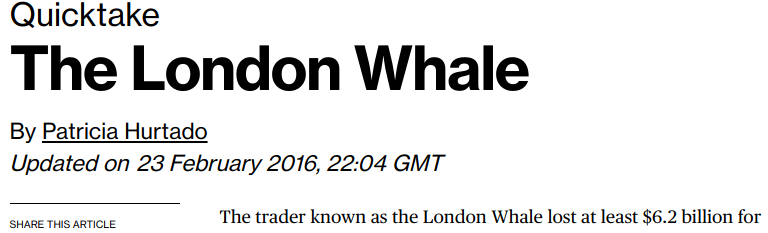
\includegraphics[width=50mm]{snafu2.jpg}};
			\pause
		    \node[drop shadow,xshift=75mm,yshift=-38mm,rotate=-35,anchor=north west] 
				at (current page.north west){
\includegraphics[width=50mm]{snafu3.jpg}};
			\pause
		    \node[drop shadow,xshift=75mm,yshift=-38mm,rotate=35,anchor=north west] 
				at (current page.north west){
\includegraphics[width=50mm]{snafu4.jpg}};
			\pause
		    \node[drop shadow,xshift=40mm,yshift=-33mm,rotate=15,anchor=north west] 
				at (current page.north west){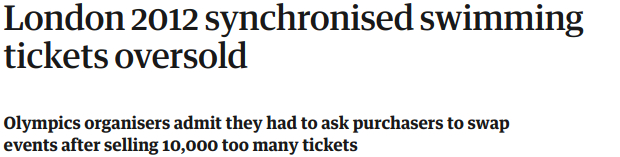
\includegraphics[width=50mm]{snafu5.jpg}};
			\pause
		    \node[drop shadow,xshift=55mm,yshift=-18mm,rotate=15,anchor=north west] 
				at (current page.north west){
\includegraphics[width=50mm]{snafu6.jpg}};
			\pause
		    \node[drop shadow,xshift=55mm,yshift=-28mm,rotate=5,anchor=north west] 
				at (current page.north west){
\includegraphics[width=50mm]{snafu7.jpg}};
			\pause
		    \node[drop shadow,xshift=35mm,yshift=-28mm,rotate=-17,anchor=north west] 
				at (current page.north west){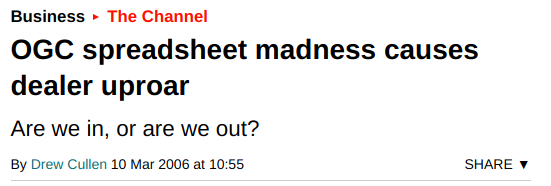
\includegraphics[width=50mm]{snafu8.jpg}};
			\pause
		    \node[drop shadow,xshift=35mm,yshift=-08mm,rotate=0,anchor=north west] 
				at (current page.north west){
\includegraphics[width=90mm]{snafu9.jpg}};
		\end{tikzpicture}
	\end{frame}
	
	\begin{frame}
		\begin{center}
			\huge
			\textbf{Spreadsheets rule the world!}
		\end{center}
	\end{frame}
	
	\begin{frame}{How you should be feeling right now}
		\begin{center}
    		\inlineMovie[loop&autostart&start=0&stop=12]{kermit.mpg}{kermit-0.png}{height=0.9\textheight}
		\end{center}
	\end{frame}

	\section{Lets draw up a battle plan}

	\begin{frame}{\mbox{}}
		\begin{center}
			\huge
			How are we going to win this?\\[2cm]
			\pause
			We are not!
		\end{center}
	\end{frame}

\end{document}
